\section{Dokumentáció}\label{sec:dokumentacio}

\subsection{Logikai adatfolyam-diagramok}

\begin{figure}[!htb]

    \centering
    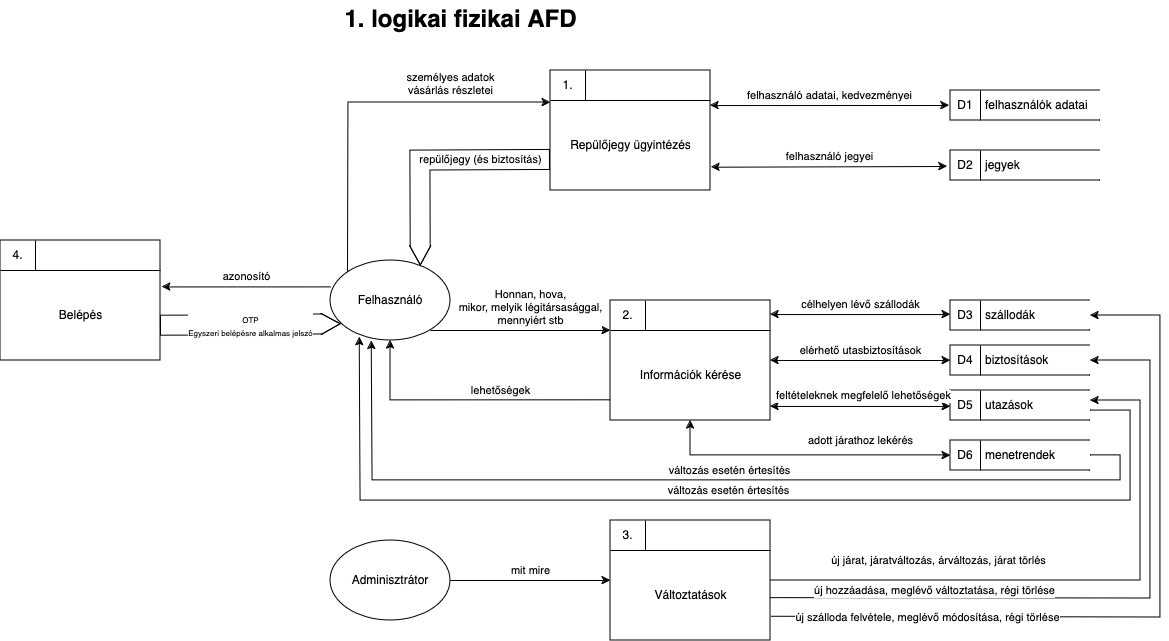
\includegraphics[scale=0.37]{logical1}
    \caption{\label{fig:logical1}Logikai AFD 1. szinten}

\end{figure}

\begin{figure}[!htb]

    \centering
    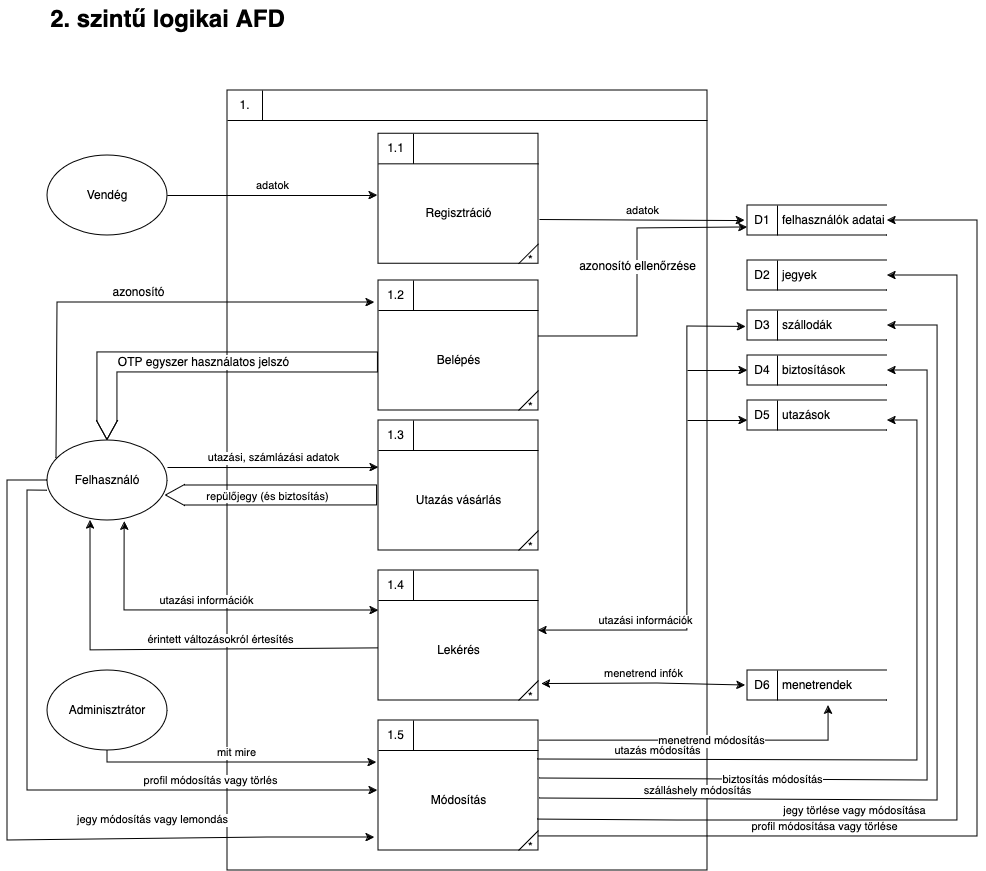
\includegraphics[scale=0.37]{logical2}
    \caption{\label{fig:logical2}Logikai AFD 2. szinten}

\end{figure}
\pagebreak

\subsection{Fizikai adatfolyam-diagramok}

\begin{figure}[!htb]

    \centering
    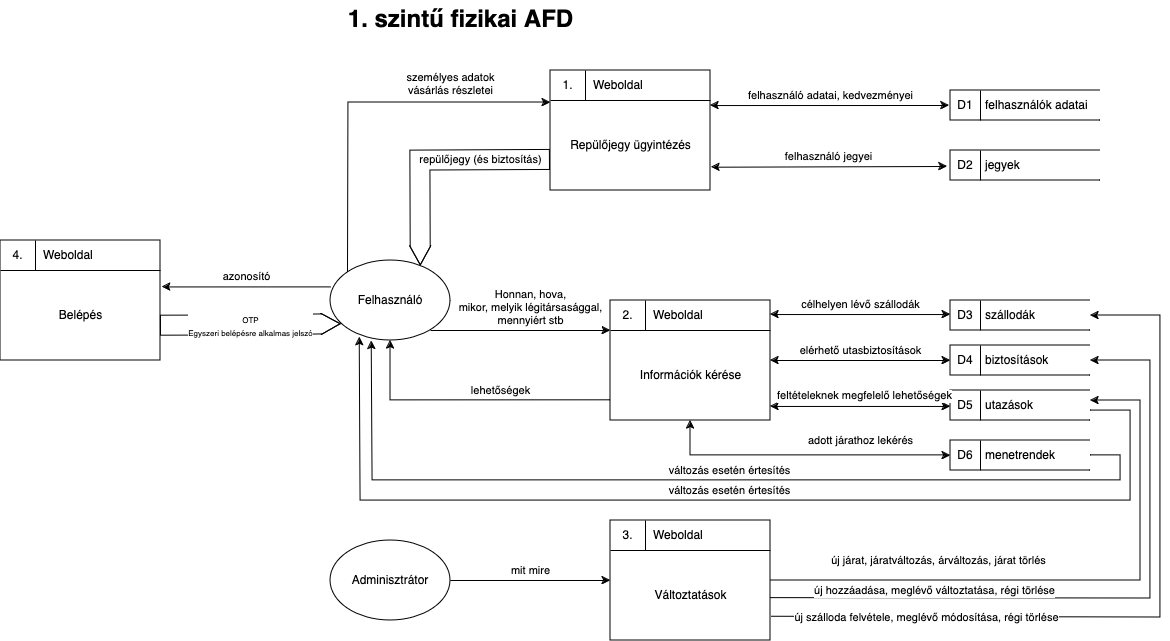
\includegraphics[scale=0.37]{physical1}
    \caption{\label{fig:physical1}Fizikai AFD 1. szinten}

\end{figure}

\begin{figure}[!htb]

    \centering
    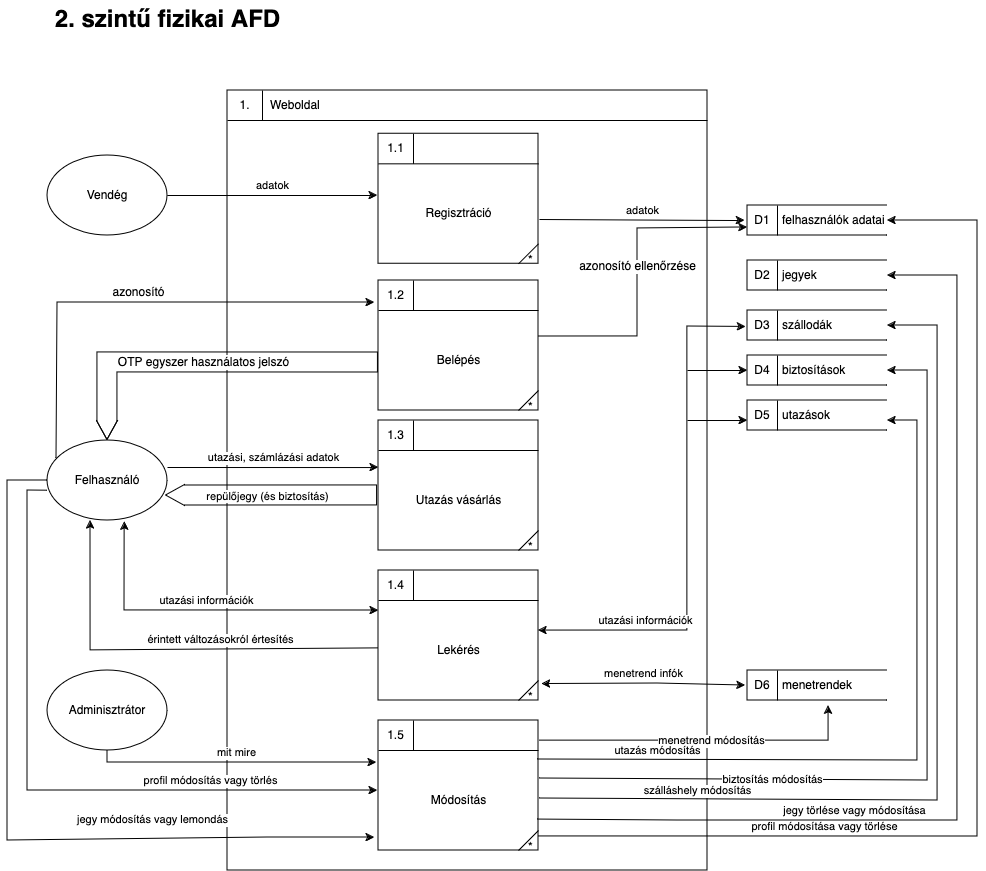
\includegraphics[scale=0.37]{physical2}
    \caption{\label{fig:physical2}Fizikai AFD 2. szinten}

\end{figure}
\pagebreak
\subsection{Egyedmodell}
\pagebreak
\subsection{E-K Diagram}

\begin{figure}[!htb]

    \centering
    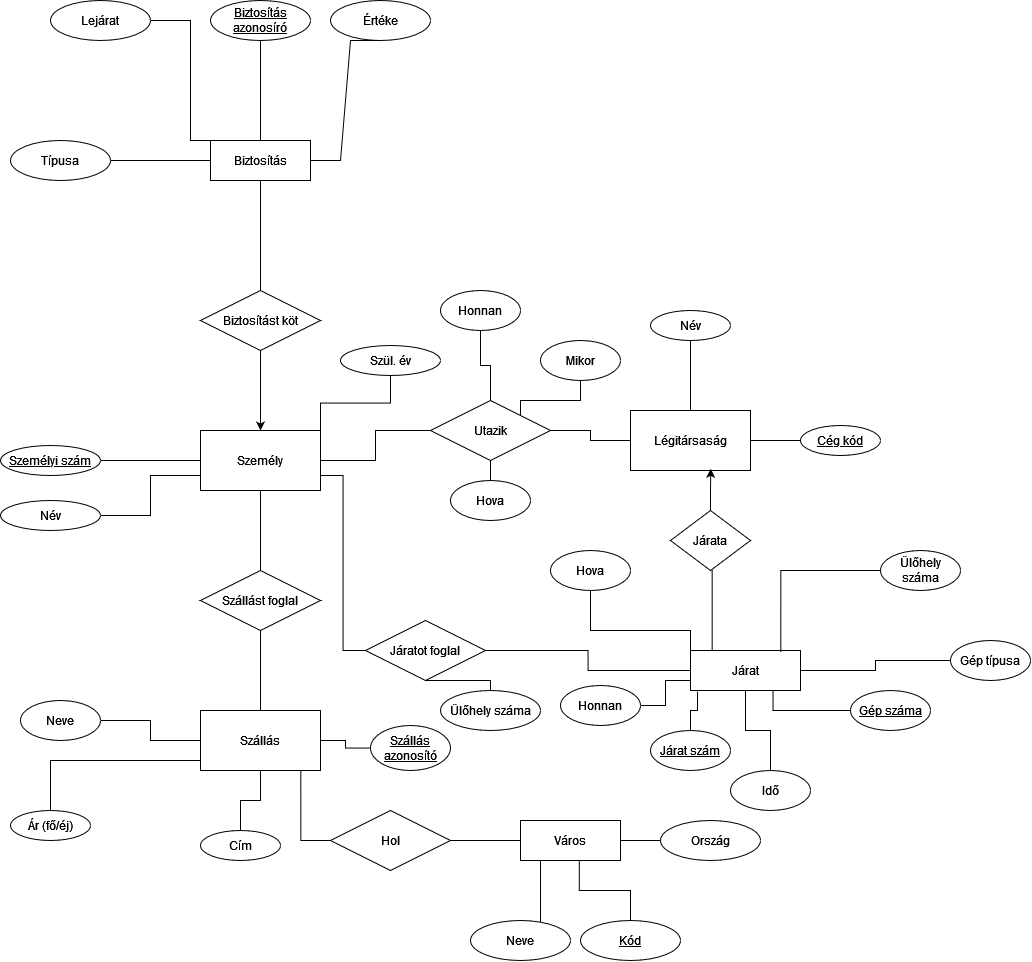
\includegraphics[scale=0.40]{e-k_diagram}
    \caption{\label{fig:e-k_diagram}E-K Diagram}

\end{figure}
\pagebreak
\subsection{Egyed-kapcsolat diagram leképezése relációs sémákká}

    BIZTOSÍTÁS(\underline{Biztosítás azonosító},Típus, Lejárat, Értéke)\\
    SZEMÉLY(\underline{Személyi szám}, Név, Szül. év)\\
    SZÁLLÁS(\underline{Szállás azonosító}, Neve, Ár (fő/éj), Cím)\\
    VÁROS(\underline{Kód} ,Neve, Ország)\\
    LÉGITÁRSASÁG(\underline{Cég kód}, Név)\\
    JÁRAT(\underline{Járat szám},\underline{Gép száma}, Hova, Honnan, Idő, Gép típusa, Ülőhely száma)

\subsection{Normalizálás (kulcsok meghatározása, alulról felfelé és felülről lefelé történő elemzés)}

\{ SZ.személyi szám \} $\rightarrow$ \{ SZ.név, SZ.születési idő\} \\
\{ LÉG.cég kód \} $\rightarrow$ \{ LÉG.név\} \\
\{ JÁR.szám \} $\rightarrow$ \{ JÁR.honnan, JÁR.hova, JÁR.gép típusa, JÁR. gép száma, JÁR.idő, JÁR.ülőhelyek száma, VÁR.kód, VÁR.neve, VÁR.ország \} \\
\{ JÁR.gép száma \} $\rightarrow$ \{ JÁR.gép típusa, JÁR.ülőhelyek száma \} \\
\{ SZÁL.azonosító \} $\rightarrow$ \{ SZÁL.neve, SZÁL.cím, SZÁL.ár, VÁR.neve, VÁR.ország \} \\
\{ VÁR.kód \} $\rightarrow$ \{ VÁR.neve, VÁR.ország \} \\
\{ BIZT.azonosító \} $\rightarrow$ \{ BIZT.biztosítás értéke, BIZT.biztosítás típusa, BIZT.lejárata \} \\
BIZTOSÍTÁS(\underline{Biztosítás azonosító},Típus, Lejárat, Értéke)\\
SZEMÉLY(\underline{Személyi szám}, Név, Szül. év)\\
SZÁLLÁS(\underline{Szállás azonosító}, Neve, Ár (fő/éj), Cím)\\
VÁROS(\underline{Kód} ,Neve, Ország)\\
LÉGITÁRSASÁG(\underline{Cég kód}, Név)\\
JÁRAT(\underline{Járat szám}, Hova, Honnan, Idő)\\
GÉP(\underline{Gép száma}, Gép típusa, Ülőhelyek száma)\\
UTAZÁS(\underline{Személyi szám}, \underline{Járat szám}, Ülés szám)
